\documentclass[a4paper,12pt]{article}
\usepackage{latexsym}
\usepackage[MeX]{polski}
\usepackage[utf8]{inputenc}
\usepackage{graphicx}
\usepackage{pdfpages}

\makeatletter
\newcommand{\linia}{\rule{\linewidth}{0.4mm}}
\renewcommand{\maketitle}{\begin{titlepage}
    \vspace*{1cm}
    \begin{center}\small
    Uniwersytet Mleczny w Gdańsku\\
    Wydział Matematyki, fizyki i informatyki\\
    \end{center}
    \vspace{4cm}
    \noindent\linia
    \begin{center}
      \LARGE \textsc{\@title}
         \end{center}
     \linia
    \vspace{0.5cm}
    \begin{flushright}
    \begin{minipage}{5cm}
    \textit{\small Autor:}\\
    \normalsize \textsc{\@author} \par
    \end{minipage}
    \vspace{2cm}
     {\small Praca wykonana pod przewodnictwem:}\\
         dr Oskyr Konkielski
     \end{flushright}
    \vspace*{\stretch{6}}
    \begin{center}
    \@date
    \end{center}
  \end{titlepage}%
}

% Zdefiniowanie autora i~tytułu:
\author{Oskar~Kąklewski}
\title{\textbf{Matematyka,~mleko~i~Kirchhoff}}
\frenchspacing
\begin{document}
% Wstawienie autora i~tytułu do składu:
\maketitle
\newpage
% Wstawienie spisu treści:
\tableofcontents
\newpage
\section{Matematyka}
\subsection{Wprowadzenie do liczb zespolonych}

Liczby zespolone wprowadzono z konieczności wyciągania pierwiastków z liczb ujemnych.
Przez całą szkołę średnią wmawia się uczniom, że "nie wolno wyciągać pierwiastka z liczby ujemnej!". Prawda ta zostaje całkowicie zburzona, gdy zaczynamy poznawać liczby zespolone. Dowiadujemy się wówczas, że:

\begin{equation}
\sqrt{-1}=\textit{i}
\end{equation}

Czy to znaczy, że przez kilkanaście lat szkolnej edukacji byliśmy oszukiwani? Nie do końca. W realnym świecie w którym żyjemy nie występują przecież żadne liczby zespolone. Każdą wielkość fizyczną, którą jesteśmy w stanie zmierzyć, możemy zawsze wyrazić za pomocy liczb rzeczywistych. W naszym normalnym, rzeczywistym świecie nie istnieją jakieś niestworzone liczby urojone...

Można więc zadać sobie pytanie, po co ludzie wymyślili coś takiego jak liczby zespolone, skoro nie istnieją one w realnym świecie. Odpowiedź jest dość prosta. Bez nich nie dałoby się wielu przydatnych rzeczy (ze świata realnego) obliczyć.
Liczby zespolone są bardzo przydatnym narzędziem, które daje nam nowe możliwości obliczeniowe. Matematyk może na chwilę opuścić nasz realny świat, udać się do świata urojonego, tam wykonać różne magiczne działania, a następnie wrócić "na ziemię" z całkowicie rzeczywistym wynikiem.

\includegraphics{mat.png}

Gdy już zaakceptujemy istnienie liczb zespolonych, to dobrze byłoby gdybyśmy nauczyli się po nich poruszać (tzn. wykonywać na nich obliczenia). Do tego celu wystarczy przyjąć, że pierwiastek z -1 jest równy tzw. jednostce urojonej~\cite{pa}, którą umówiono się oznaczać literką i. Zapiszmy zatem jeszcze raz tą kluczową równość:

\begin{equation}
\sqrt{-1}=\textit{i}
\end{equation}

Zauważmy od razu, że równoważna jest jej następująca równość:

\begin{equation}
\textit{i}^{2}=-1
\end{equation}

Powyższe wiadomości oraz wiedza ze szkoły średniej (umiejętność wykonywania działań na wyrażeniach algebraicznych, potęgowania, pierwiastkowania, znajomość wzorów skróconego mnożenia, itp.) pozwolą na wykonywanie wszystkich podstawowych działań na liczbach zespolonych. Ale jak dokładnie wyglądają te liczby zespolone? Każdą liczbę zespoloną można przedstawić jako sumę liczby rzeczywistej i urojonej (jest to takie zespolenie świata rzeczywistego i świata czysto urojonego~\cite{pa}).

\subsection{Definicja liczby zespolonej}

Liczbą zespoloną nazywamy liczbę postaci:

\begin{equation}
\textit{a}+\textit{bi}
\end{equation}

gdzie \textit{a}, \textit{b} - to dowolne liczby rzeczywiste.

Zauważ, że jeżeli weźmiemy \textit{b} = 0, to otrzymamy zwykłą liczbę rzeczywistą. Jeżeli natomiast weźmiemy \textit{a} = 0, to otrzymamy liczbę zespoloną, która będzie czysto urojona (tzn. nie bedzie mieć części rzeczywistej).

Przykłady:

\begin{enumerate}
  \item liczb zespolonych z częścią rzeczywistą i urojoną:
  5+\textit{i}, 3+9\textit{i}
  \item liczb zespolonych tylko z częścią urojoną:
  2\textit{i}, 5\textit{i}
\end{enumerate}

\section{Mleko}
Mleko to wydzielina gruczołu mlekowego samic ssaków pojawiająca się w okresie laktacji. Jako produkt żywnościowy dla człowieka największe znaczenie ma mleko krowie. Według Międzynarodowej Federacji Mleczarskiej mleko krowie jest produktem całego, nieprzerwanego doju, od zdrowej, dobrze żywionej krowy mlecznej, otrzymany w sposób prawidłowy.

Mleko jest mieszaniną wieloskładnikową; składająca się z trzech podstawowych faz (te trzy fazy znajdują się w ścisłej zależności-interakcji):

\begin{itemize}
  \item emulsyjnej
  \item koloidalnej
  \item molekularnej
\end{itemize}

Średni skład mleka u różnych ssaków (g/100 ml):


\begin{tabular}{ l || c | r }
  \textbf{Gatunek} & \textbf{Tłuszcz} & \textbf{Białko} \\
  Słoń & 22,1 & 3,2 \\
  Szympans & 3,7 & 1,2 \\
  Człowiek & 4,0 & 1,3 \\
  Koń & 1,6 & 2,7 \\
  Owca & 9,0 & 4,7 \\
\end{tabular}

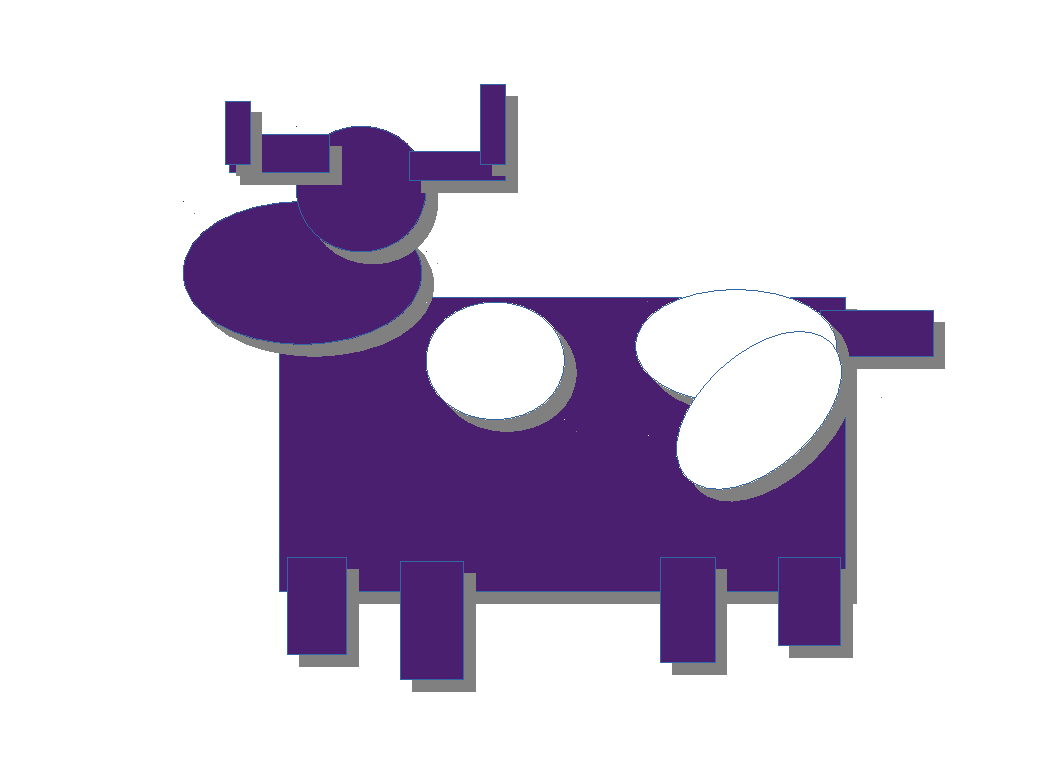
\includepdf[pages={1}]{Krowa_mala.pdf}

\section{Kirchhoff}
Prądowe prawo Kirchhoffa:
\begin{equation}
\sum_{k=1}{n} I_k = 0 \; .
\end{equation}

\section{Tabela}
\begin{tabular}{|r|l|}
  \hline
  To & tylko \\
  \hline
  \hline
  inny & rodzaj \\
  \hline
  tabeli & :) \\
  \hline
\end{tabular}

\begin{thebibliography}{99}
\bibitem{pa} H.~Partl:
\emph{German \TeX},
TUGboat Vol.~9,nr~1 ('88)
\bibitem{pa} O.~Konklewski:
\emph{Polish \TeX},
Mleko, nr~1 ('78)
\end{thebibliography}
\end{document}
